\documentclass[twoside]{article}
\usepackage{graphicx}
\usepackage[top=2.5cm,left=2.5cm,right=2.5cm,bottom=2.5cm,headsep=0.3in,headheight=1in]{geometry}
\usepackage{multirow}
\usepackage[ngerman]{babel}
\usepackage{float}
\usepackage{fancyhdr}
\usepackage{minted}
\usepackage{hyperref}
\setminted{
	autogobble,								% rückt Code soweit nach links wie möglich
	stepnumber=2,							% nur jede gerade Zeilennummer wird angezeigt
	fontfamily=tt,
	linenos=true,
	numberblanklines=true,
	numbersep=5pt,
	gobble=0,
	frame=single,
	framerule=0.4pt,
	framesep=2mm,
	funcnamehighlighting=true,
	tabsize=4,
	obeytabs=false,
	breaklines,
	breakafter=">/,
	breakbefore=. ,
	breaksymbolindentright=10pt,
	breaksymbolsepright=0pt
}
\usepackage{amsmath}
\usemintedstyle{vs}


%Eingabe der Parameter in die letzten geschwungenen Klammern

\newcommand{\titeltitel}{Bluetooth}                  %Titel der Übung
\newcommand{\titelraumbezeichnung}{}        %Raumbezeichnung
\newcommand{\titelgruppe}{E}                 %Gruppe
\newcommand{\titellehrer}{LAP}                 %Lehrer
\newcommand{\titeluebungsnummer}{2}          %Übungsnummer
\newcommand{\titelabgabedatum}{24.01.2025}            %Abgabedatum
\newcommand{\titelkatalognummer}{25}          %Katalognummer
\newcommand{\titeluebungdatum}{17.01.2025}            %Übungsdatum
\newcommand{\titelnameprotokoll}{Reichart Florian}          %Name des Protokollist
\newcommand{\titelnameteam}{Mayer Phillip}               %Name der Teammitglieder
\newcommand{\titelklasse}{5BHEL}                 %Klasse
\newcommand{\titelgeprueftdatum}{}          %Prüfungsdatum  %Definiert Variablen für das Titelblatt

\begin{document}

%Titelblatt
\thispagestyle{empty}
\newgeometry{top=20mm, left=18.25mm, right=18.25mm, bottom=20mm}
\noindent
\begin{tabular}{|p{4.5cm}|p{7.5cm}|p{2.5cm}|p{2cm}|} %17.35mm
    \hline
    \vspace{0.4cm}
    \multirow{2}{4.5cm}{\hspace{0.7cm}
\includegraphics{img/titel/Labor_Protokoll_Logo.jpg}} & \multirow{2}{7.5cm}{\begin{center}{\huge Laboratorium}\\\vspace{0.25cm} Raumbezeichnung: \hspace{0.25cm} \titelraumbezeichnung \end{center}} & \vspace{0.05cm} Katalognummer:\vspace{0.3cm} & \vspace{0.06cm}\hspace{0.7cm}{\Large\titelkatalognummer}\\
    \cline{3-4}
     & & \vspace{0.05cm}Tag der Übung:\vspace{0.3cm} & \vspace{0.14cm} {\large\titeluebungdatum} \\
    \hline
    \vspace{0.35cm} {\large Gruppe: \titelgruppe} & \vspace{0.1cm} {Protokoll: \hspace{0.27cm} \titelnameprotokoll \vspace{0.1cm} \newline Mitglieder: \hspace{0.1cm} \titelnameteam} \vspace{0.2cm} & \vspace{0.35cm} {\large Klasse} & \vspace{0.35cm} {\Large\titelklasse} \\
    \hline
    \multicolumn{4}{|p{17cm}|}{%Bei Bild vspace unten ändern
    \vspace{18cm}}\\
    \hline
\end{tabular}

\vspace{-1px}
\noindent
\begin{tabular}{|p{2.3cm}|p{1.8cm}|p{7.9cm}|p{2.5cm}|p{1.58cm}|}
    \vspace{0.1cm}Lehrer\vspace{0.2cm} & \vspace{0.1cm}\titellehrer & \vspace{0.15cm} \multirow{2}{7.1cm}{\centerline{Titel der Übung}\vspace{0.2cm}\newline\centerline{\huge \textbf{\titeltitel}}} & \vspace{0px} Übungsnummer & \vspace{1px}\titeluebungsnummer\\
    \cline{1-2}\cline{4-5}
    \vspace{0px}Geprüft\vspace{0.15cm} & \vspace{0px} \titelgeprueftdatum &  & \vspace{0px}Abgabe am\vspace{0.15cm} & \vspace{0px}\titelabgabedatum \\
    \hline
\end{tabular}
\newgeometry{top=2.5cm,left=2.5cm,right=2.5cm,bottom=2.5cm,headsep=0.3in,headheight=1in}

%Kopf- und Fußzeile
\pagestyle{fancy}
\fancyhead[R]{\titelnameprotokoll} %Protokollist oben rechts
\fancyhead[L]{\titeluebungdatum}   %Übungsdatum oben links
\fancyfoot[C]{\titeltitel}         %Titel der Übung unten mittig
\fancyfoot[R]{\thepage}           %Seitennummer unten außen

%Inhaltsverzeichnis
\tableofcontents
\newpage

%Begin der Dokumentation
\section{Aufgabe 1: Bluetooth-Lautsprecher}
\subsection{Aufgabenstellung}
In dieser Aufgabe soll der ESP32 als Bluetooth-Lautsprecher fungieren. Dafür soll die Arduino IDE mit der fertigen Bibliothek von pschatzmann (\href{https://github.com/pschatzmann/ESP32-A2DP}{Quelle}) verwendet werden. Um die Funktion zu überprüfen, soll ein Lautsprecher an den ESP32 angeschlossen werden.

\subsection{Aufbau}
\begin{figure}[h]
    \centering
    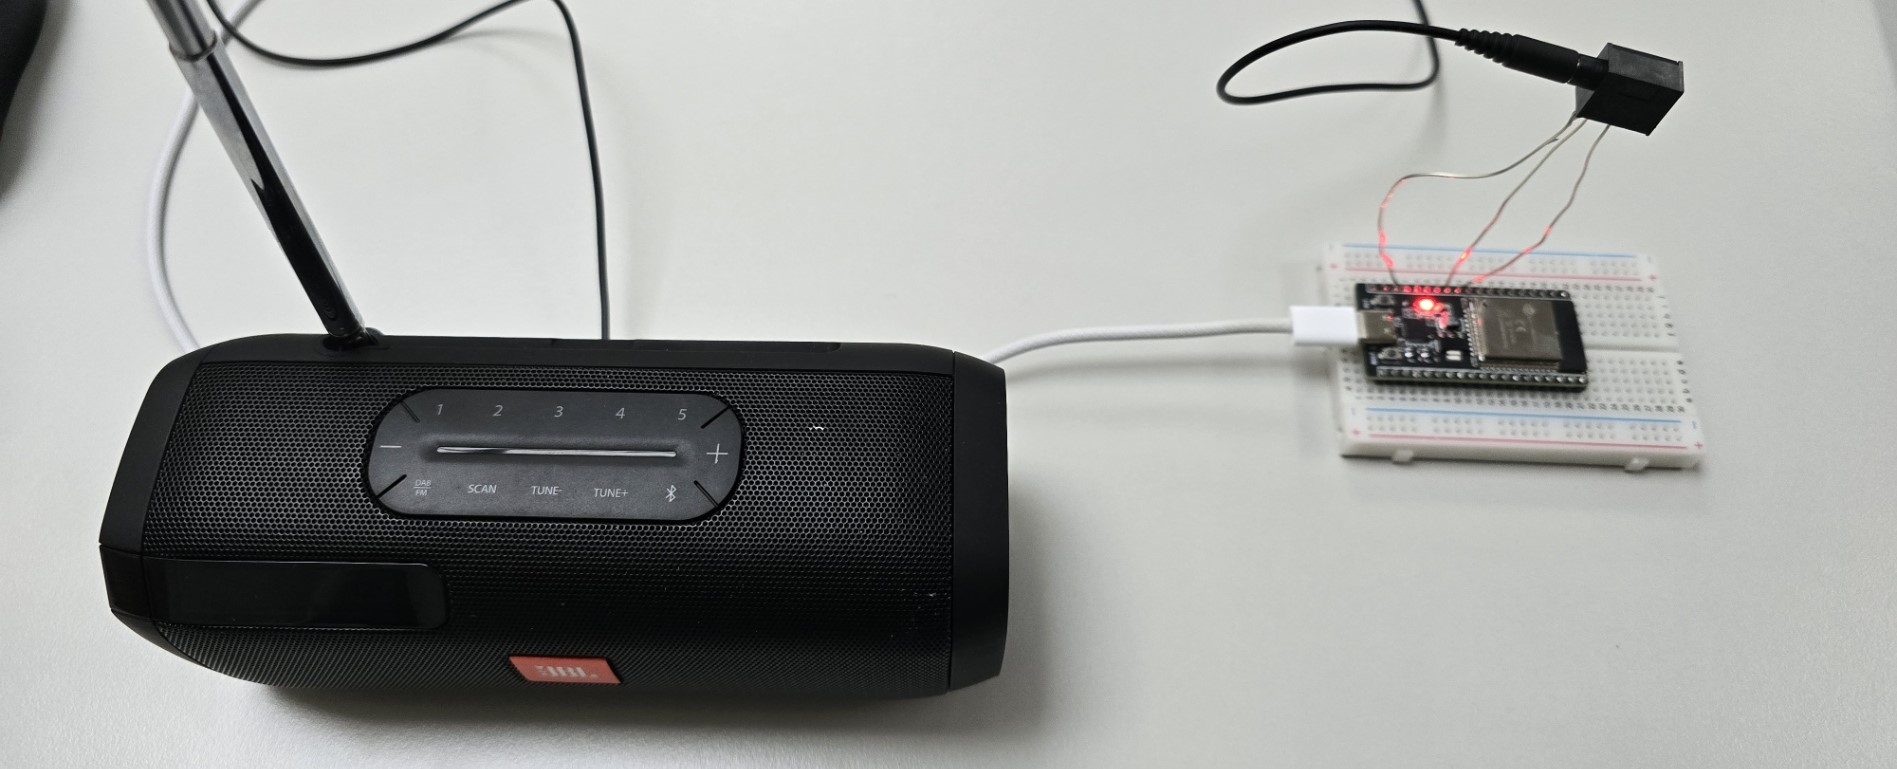
\includegraphics[width=0.9\linewidth]{img/Aufbau_01.jpg}
\end{figure}

\subsection{Installation der Bibliothek}
Im Readme der Bibliothek wird die Installation beschrieben. Zuerst muss man den \textit{libraries}-Ordner der Arduino IDE öffnen. Dieser befindet sich standardmäßig unter \textit{Documents/Arduino/libraries} und kann bei Bedarf auch in der Arduino IDE ausgelesen werden.
\begin{figure}[h]
    \centering
    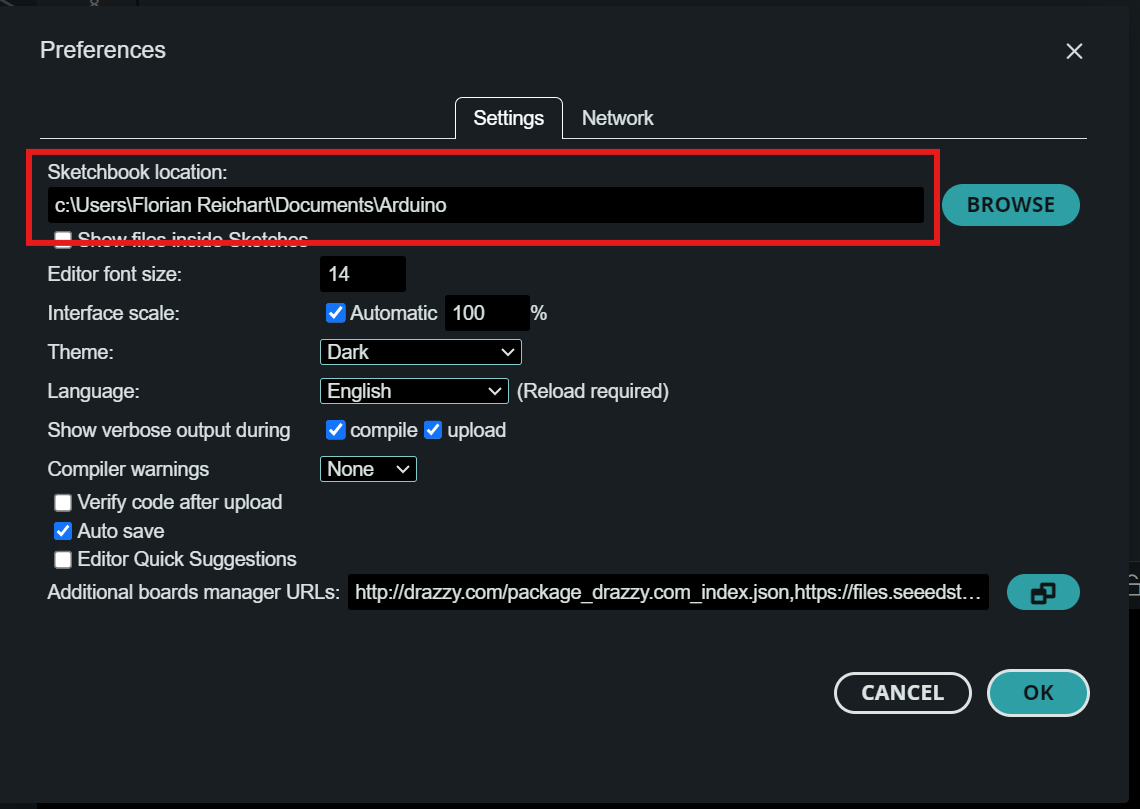
\includegraphics[width=0.5\linewidth]{img/Arduino_IDE_Pref_01.png}
\end{figure}
Nachdem dieser Ordner geöffnet wurde, müssen in ihm zwei Befehle ausgeführt werden. Wenn der Ordner im Windows-Explorer geöffnet wurde, kann in der Adressleiste der Befehl \textit{cmd} eingegeben werden.
\begin{figure}[h]
    \centering
    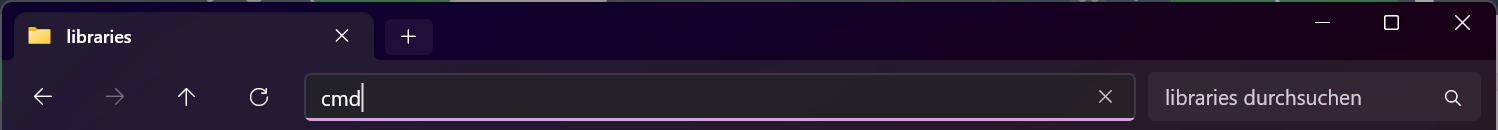
\includegraphics[width=1\linewidth]{img/Explorer_01.png}
\end{figure}
\\
Im Befehlsfenster müssen nun folgende Befehle eingegeben werden:
\begin{minted}{bash}
git clone https://github.com/pschatzmann/ESP32-A2DP.git
git clone https://github.com/pschatzmann/arduino-audio-tools.git
\end{minted}
Somit sollten die Bibliotheken installiert und nutzbar sein.

\subsection{Programmcode}
Der folgende Programmcode stammt aus dem GitHub der Bibliothek.

\begin{minted}{cpp}
#include "AudioTools.h"
#include "BluetoothA2DPSink.h"

AnalogAudioStream out;
BluetoothA2DPSink a2dp_sink(out);

void setup() {
    a2dp_sink.start("ReichartMayer");
}

void loop() {
}
\end{minted}

\subsection{Hochladen des Codes}
Um den Code erfolgreich auf den ESP32 hochzuladen, muss das Aufteilungsschema des Speichers geändert werden. Dies kann unter `Tools` durchgeführt werden.
\begin{figure}[h]
    \centering
    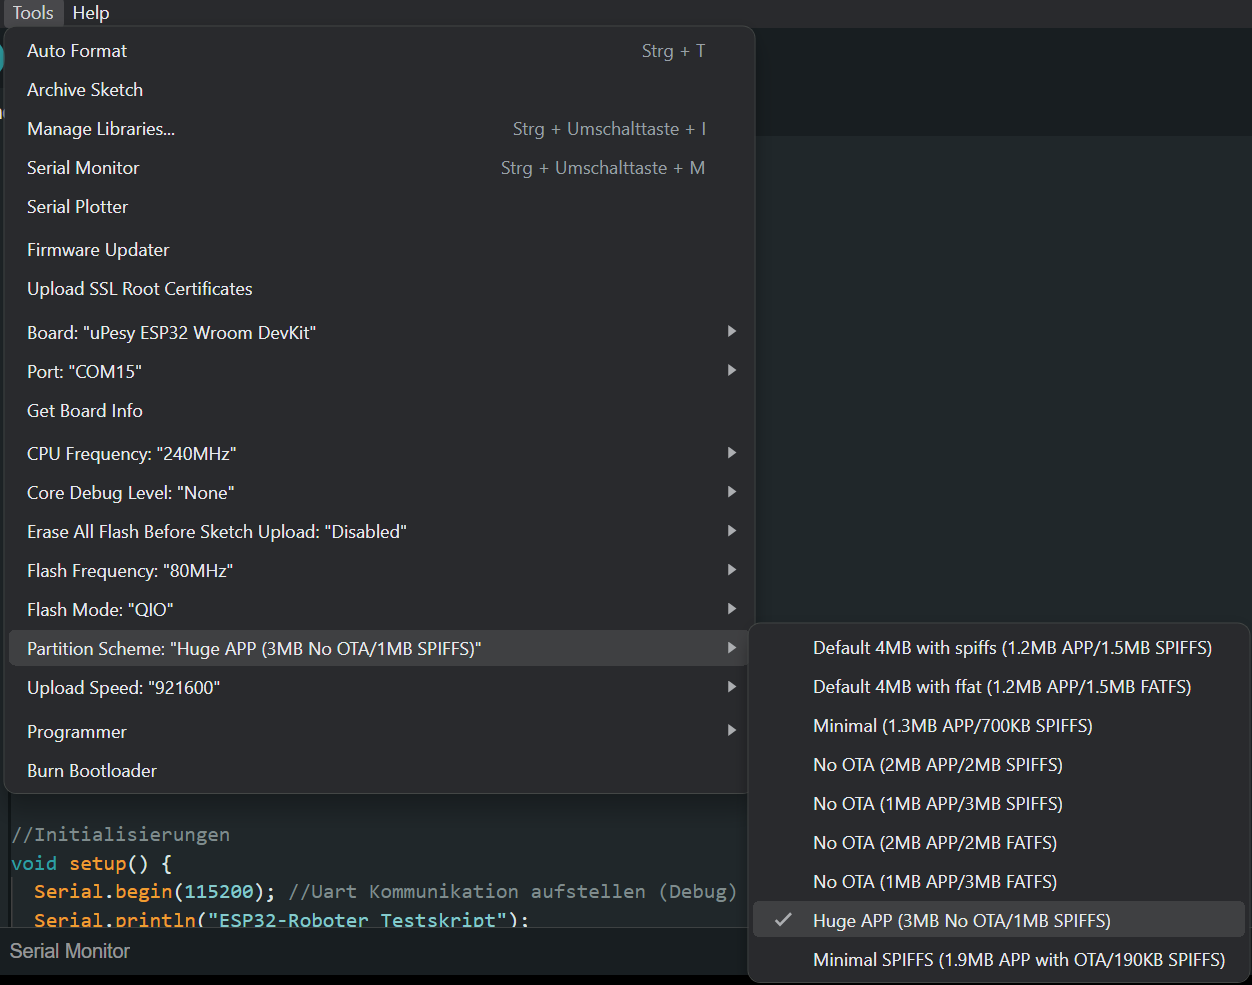
\includegraphics[width=0.55\linewidth]{img/Arduino_IDE_02.png}
\end{figure}

\subsection{Test des Codes}
Nachdem der Code hochgeladen wurde, wurde der Lautsprecher mit dem Klinkenstecker mit dem ESP32 verbunden. Anschließend wurde der ESP32 über Bluetooth mit einem Smartphone gekoppelt. Der ESP32 wird als "ReichartMayer" angezeigt, da dies der Startfunktion mitgegeben wurde. Nach der erfolgreichen Kopplung wurde Musik am Smartphone abgespielt, welche am Lautsprecher wiedergegeben wurde.

\newpage
\section{Aufgabe 2: iBeacon mit dem ESP32}
\subsection{Aufgabenstellung}
In dieser Aufgabe soll ein iBeacon mit dem ESP32 erstellt werden. Dieser soll in regelmäßigen Abständen Daten aussenden. Um die Daten zu empfangen, wird die App \textit{nRF Connect} von NORDIC Semiconductor aus dem App Store verwendet.

\subsection{Grundlagen von iBeacon}
iBeacon ist eine von Apple entwickelte Technologie, die auf Bluetooth Low Energy (BLE) basiert und präzise Standorterkennung in Innenräumen ermöglicht. Dabei senden kleine Sender, sogenannte Beacons, Signale aus, die von kompatiblen Geräten wie Smartphones empfangen werden können. Diese Signale enthalten Informationen, die es Anwendungen erlauben, kontextbezogene Aktionen auszulösen, zum Beispiel das Anzeigen von Angeboten in Geschäften, die Navigation in Gebäuden oder die Automatisierung von Prozessen. Die Technologie zeichnet sich durch ihre Energieeffizienz, einfache Implementierung und vielseitige Einsatzmöglichkeiten im Einzelhandel, in Museen oder auf Messen aus.

\subsection{Programmcode}
Der folgende Code stammt von N3MIS15 (\href{https://gist.github.com/N3MIS15/589062360a658a36b9c810fec8bb0c91}{Quelle}). Jedoch wurden die Bytes der uuid angepasst, um im ASCII-Code-Format den String \textit{ReichartMayerLab} anzuzeigen.
\begin{minted}{python}
import struct
import ubluetooth as bt
from micropython import const

MANUFACTURER_ID         = const(0x004C)
DEVICE_TYPE             = const(0x02)
DATA_LENGTH             = const(0x15)
BR_EDR_NOT_SUPPORTED    = const(0x04)
FLAG_BROADCAST          = const(0x01)
MANUFACTURER_DATA       = const(0xFF)

def convert_tx_power(dbm):
    return dbm + 0xFF + 1

class iBeacon():
    def __init__(self, ble, uuid, major, minor, tx_power):
        # Setup BLE
        self.ble = ble
        self.ble.active(False)
        self.ble.active(True)
        print("BLE Activated")

        self.uuid = uuid
        self.major = major
        self.minor = minor
        self.tx_power = convert_tx_power(tx_power)
        self.adv_payload = self.create_payload()


    def create_payload(self):
        payload = bytearray()
            
        #Set advertising flag
        value    = struct.pack('B', BR_EDR_NOT_SUPPORTED)
        payload += struct.pack('BB', len(value) + 1, FLAG_BROADCAST) + value

        # Set advertising data
        value    = struct.pack('<H2B', MANUFACTURER_ID, DEVICE_TYPE, DATA_LENGTH) 
        value   += self.uuid
        value   += struct.pack(">2HB", self.major, self.minor, self.tx_power)
        payload += struct.pack('BB', len(value) + 1, MANUFACTURER_DATA) + value

        return payload


    def advertise(self, interval_us=100000):
        print("Advertising: " + str(self.adv_payload))
        self.ble.gap_advertise(None)
        self.ble.gap_advertise(interval_us, adv_data=self.adv_payload, connectable=False)


    def update(self, major, minor, advertise_interval):
        self.ble.active(False)

        self.major = major
        self.minor = minor
        self.adv_payload = self.create_payload()

        self.ble.active(True)
        self.advertise(advertise_interval)


def demo():
    beacon = iBeacon(
        ble         = bt.BLE(), 
        uuid        = bytearray((
                        0x52, 0x65, 0x69, 0x63, 0x68, 0x61, 0x72, 0x74, 
                        0x4d, 0x61, 0x79, 0x65, 0x72, 0x4c, 0x61, 0x62
                    )),
        major       = 62,
        minor       = 1050,
        tx_power    = -50,
    )

    beacon.advertise()

if __name__ == "__main__":
    demo()
    while True:
        pass
\end{minted}

\subsection{Test des Programms}
Nachdem der Code auf den ESP32 hochgeladen wurde, wurde die nRF Connect App geöffnet. Dort wurde ein iBeacon-Gerät entdeckt. Nachdem Details über das Gerät angezeigt wurden, wurde erkannt, dass die UUID des Geräts mit der im Code eingestellten übereinstimmt und es sich somit um das selbst programmierte Gerät handelt.
\begin{figure}[h]
    \centering
    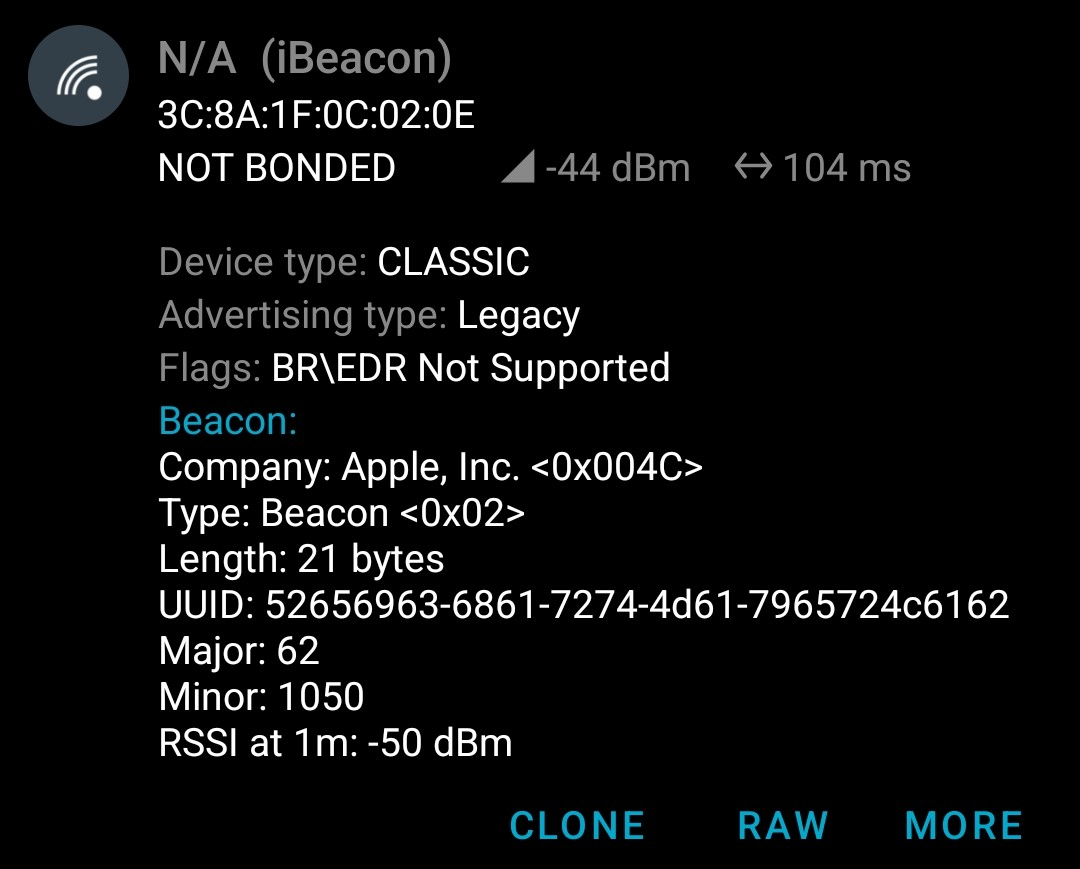
\includegraphics[width=0.5\linewidth]{img/nRF_01.jpg}
    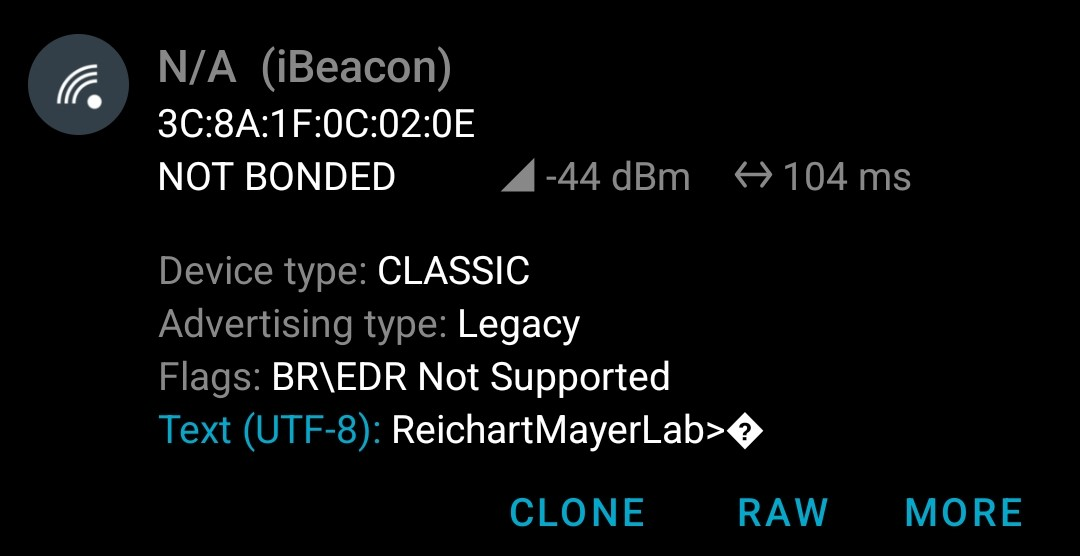
\includegraphics[width=0.5\linewidth]{img/nRF_02.jpg}
\end{figure}
\newpage
\section{Aufgabe 3: Remote ID einer Drohne}
\subsection{Aufgabenstellung}
In dieser Aufgabe soll die Remote ID einer kommerziellen Drohne empfangen und angezeigt werden.

\subsection{Programmcode}
\begin{minted}{cpp}
#include <BLEDevice.h>
#include <BLEUtils.h>
#include <BLEScan.h>
#include <BLEAdvertisedDevice.h>
 
BLEScan* pBLEScan;
int scanTime = 10;
 
void setup() {
  Serial.begin(115200);
  Serial.println("Starting BLE scan...");
  BLEDevice::init("");
  pBLEScan = BLEDevice::getScan();
  pBLEScan->setActiveScan(true);
  pBLEScan->setInterval(100);
  pBLEScan->setWindow(99);
  pBLEScan->start(scanTime, scanComplete);
}
 
void loop() {
  delay(1000);
}
 
void scanComplete(BLEScanResults scanResults) {
  Serial.print("Scan complete, found ");
  Serial.print(scanResults.getCount());
  Serial.println(" devices");
 
  for (int i = 0; i < scanResults.getCount(); i++) {
    BLEAdvertisedDevice device = scanResults.getDevice(i);
    Serial.print("Device Name: ");
    Serial.println(device.getName().c_str());
    Serial.print("Device Address: ");
    Serial.println(device.getAddress().toString().c_str());
    Serial.print("RSSI: ");
    Serial.println(device.getRSSI());
    Serial.print("Tx Power: ");
    Serial.println(device.getTXPower());
    Serial.print("Service UUIDs: ");
    String serviceUUIDs = device.getServiceUUID().toString();
    Serial.println(serviceUUIDs.c_str());
    Serial.print("Manufacturer Data: ");
    if (device.haveManufacturerData()) {
      String manufacturerData = device.getManufacturerData();
      Serial.println(manufacturerData.c_str());
    }
    Serial.print("Service Data: ");
    if (device.haveServiceData()) {
      String serviceData = device.getServiceData();
      Serial.println(serviceData.c_str());
    }
    Serial.print("Appearance: ");
    Serial.println(device.getAppearance());
    Serial.println();
  }
}
\end{minted}

\subsubsection{Test des Programms}
Das Programm wurde ausgeführt und verschiedene Daten, inklusive der Remote ID, wurden von den Geräten angezeigt. Somit kann diese auch von kommerziellen Drohnen und anderen Geräten ausgelesen werden.

\section{Aufgabe 4: Dokumentation}
\subsection{Bearbeitung von LaTeX}
Latex erzeugt eine PDF, die zur visuellen Kontrolle benutzt werden kann. Um den reinen Latex-Code anzusehen und zu bearbeiten, kann ein Latex-Editor wie \href{https://www.overleaf.com}{Overleaf} genutzt werden. Nachdem dort ein Konto erstellt wurde, kann das Projekt über \textit{New Project} $\to$ \textit{Upload Project} als ZIP importiert werden.

\end{document}
